\documentclass{article}
\usepackage{graphicx} % Required for inserting images
\usepackage{tikz}
\usepackage{amsthm}
\usepackage{amssymb}
\usepackage{mathtools}
\PassOptionsToPackage{hyphens}{url}\usepackage{hyperref}

\usepackage{pgfplots}
\pgfplotsset{width=10cm,compat=1.9}

\title{15418 Final Report - Parallel SAT Solving}
\author{Liam Gersten (lgersten) and Alexander Wang (aywang)}

\begin{document}

\maketitle
\tableofcontents

\section{Summary}
We implemented an parallel CPCL-driven SAT solver using MPI and work stealing.
Our goal for the SAT solver was to quickly solve killer sudokus, where upon testing on the Bridges-2 machines, we obtained close-to-linear speedup (for $n=1,2,4,8,16$, we obtained a speedup of roughly $3/4\times$).

\section{Background}

\subsection{Killer Sudoku}
A sudoku is a pencil-and-paper number puzzle where the solver must fill in an $n \times n$ grid with numbers from 1 to $n$, where $n$ is a square number.
Traditionally, $n = 9$.
There are three main constraints in a regular sudoku puzzle: no digit may appear in the same row, column, or box, where the puzzle grid is partitioned into $n$ smaller $\sqrt{n} \times \sqrt n$ boxes.

Furthermore, the sudoku puzzle must have a unique solution.
Therefore, it is typical for several digits to be pre-inputted into the grid.

In the killer sudoku variant, no such digits are given.
In Figure~\ref{fig:sudoku_ex}, we observe cages containing a number in the upper-left corner.
Within a cage, no digit may repeat;
furthermore, the digits must sum to the number of that cage.

\begin{figure}
    \centering
    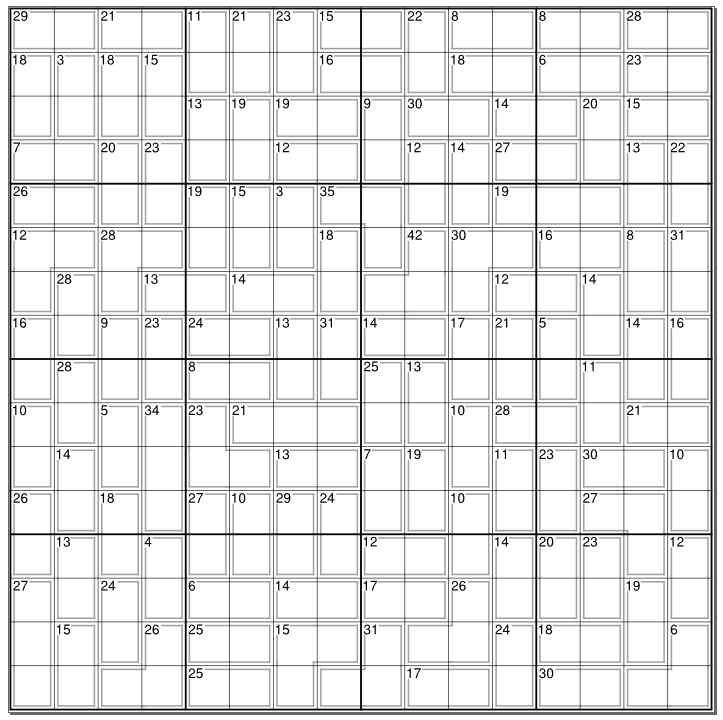
\includegraphics[width=0.8\linewidth]{images/sudoku_example.png}
    \caption{An example 16x16 killer sudoku puzzle. (Ref: \url{https://www.calcudoku.org/forum/viewtopic.php?f=19&t=731})}
    \label{fig:sudoku_ex}
\end{figure}

We kept the goal of solving killer sudokus in mind, for us to optimize our parallel SAT solving algorithm over.
Indeed, the rules of traditional sudoku easily convert to a SAT instance, however the sum constraints turn out to be much trickier, both to reduce to SAT and for our program to solve.

\subsection{Sat Reductions}

The key idea in most of the constraints are the \verb|onlyOneClauses|$(\{v_i\})$, which reduces the exactly-one constraint into SAT.
Indeed, consider the $n^3$ unary variables $v(r,c,d)$ representing the truth value of digit $d$ occupying row $r$ and column $c$.
Within each row and column, we can only have one digit; and similar for row and digit, and column and digit.
We also have \verb|onlyOneClauses| for within each box and killer cage.

The naive method is to have two flavors of clauses: $\bigvee v_i$ and $\neg (v_i \land v_j) = \neg v_i \lor \neg v_j$ for every distinct $i,j$.
Over $n$ variables, this converts to $O(n^2)$-many clauses.
However, a more clever idea is to add auxiliary variables to be able to reduce to linearly-many clauses.

In the commanding-variable encoding, for every set of 3 variables, we enforce $c_{ijk} \iff v_i \lor v_j \lor v_k$, as well as $\bigwedge_{\text{sym}} (\neg v_i \lor \neg v_j)$.
Indeed, this turns out to only require linearly many clauses ($\lceil \frac{7(n-2)}{2} \rceil$) at the cost of adding linearly many variables ($\lceil \frac{n}{2}-2 \rceil$).
We briefly note that even though we are adding more variables, this does not change the degrees of freedom of our algorithm, given that we solely case on the non-auxiliary variables.
In other words, unit propagation will always suffice in determining our commander variables.

We can slightly optimize this further.
If we split the grid into $n\sqrt{n}$-many $1 \times \sqrt{n}$ subrows, and use a commander variable to represent that, we may use the same commander variables for \verb|oneOfClauses| of both boxes and rows.
A similar mini-optimization is possible for correctly-aligned killer cages.

For killer sums, the naive way turns out to be optimal in small grid cases ($n=9,16$).
That is, per cage, we have a variable $d_c$ encode if a digit exists within a cell.
Then, we have another variable $p_c$ encode every possible set of numbers that a cell could contain.
Lastly, we add the clause $\bigvee p_c$, representing that the cell must hold (at least) one of these sets.

Of course, this is exponential in $n$.
By using variables to represent partial sums modulo small primes, we can get a loglinear number of clauses, although the constant is too large in the cases of small $n$ and small-sized cages.

\subsection{DPLL}
DPLL is the original way of solving SAT instances.
If we imagine the search space of boolean assignments as a binary tree, as in Figure~\ref{fig:dec-tree}, we can traverse the tree recursively via a standard backtracking algorithm.

The most important part of this algorithm is unit propagation, which after deciding on a variable, iteratively looks for unit clauses to satisfy.
Especially for a sudoku, with many small clauses, it is important for this functionality to be as streamlined as possible.

\subsection{CDCL}
CDCL (Conflict-Driven Clause Learning) is the algorithm which gives us a practical chance to solve harder SATs.
Whenever the algorithm runs into a contradiction, it derives a clause that would prevent it from making the same mistake down the line.
Therefore, by learning more clauses as it goes, we are able to narrow the search space more and more.
In our algorithm, we implement the 1UIP method of deriving conflict clauses, which will be described thoroughly in a following section.

\subsection{Our Approach to Parallelism}
The very first dilemma of our project was to decide if we wanted to use the Shared Address or Message Passing paradigm.
Parallel SAT is inherently challenging due to load balancing.
A priori, it is impossible to know how lopsided our search space tree is - i.e., what decisions work, what decisions fail quickly, and what decisions fail slowly?
This led us to consider a work-stealing approach, where idle processors could steal work from busy threads.
We decided on MPI because of two properties:
First, the information that a thread would need to work-steal would only be a partial assignment (and the reduced formula it entails), which requires very little memory to send.
Secondly, two threads working on different parts of the search space do not need to communicate at all between each other at all except to steal work or prematurely terminate the algorithm.

Upon our choice of MPI, we encountered many interesting problems we needed to solve, including:
\begin{itemize}
    \item A time/space tradeoff between a message's need to be compact but also fast to decode.
    \item How should processors be interconnected together?
    \item How would the threads collectively know if there is work left or not?
    \item How do we generate or handle conflict clauses? 
    \item To what capacity should we share generated conflict clauses?
\end{itemize}
These will all be detailed in the following section.

\section{Approach}

\subsection{Serial Implementation}

\subsubsection{Recursion and Unit Propagation}

\begin{figure}
    \begin{center}
        \begin{tikzpicture}
            \begin{scope}[every node/.style={circle,thick,draw}]
                \node (R) at (8, 3) {$S_0$};
                \node (S1T) at (4, 1) {$S_1$};
                \node (S1F) [dashed, draw=gray, thin, text=gray] at (12, 1) {$S_1'$} ;
                \node (S2T) [draw=orange, thin, text=orange] at (2, -1) {$S_2$};
                \node (S2F) at (7, -1) {$S_2'$} ;
                \node (S3T) at (5, -3) {$S_3$};
                \node (S3F) [dashed, draw=gray, thin, text=gray] at (9, -3) {$S_3'$} ;
            \end{scope}
            
            \begin{scope}[
                          every node/.style={fill=white,circle},
                          every edge/.style={draw=black,very thick}]
                \path [->] (R) edge[bend right=20] node {$x_1 = T$} (S1T);
                \path [->] (R) edge[bend left=20, dashed, draw=gray, thin, text=gray] node {$x_1 = F$} (S1F);
                \path [->] (S1T) edge[bend right=20, draw=orange, thin, text=orange] node {$x_2 = T$} (S2T);
                \path [->] (S1T) edge[bend left=20] node {$x_2 = F$} (S2F);
                \path [->] (S2F) edge[bend right=20] node {$x_3 = T$} (S3T);
                \path [->] (S2F) edge[bend left=20, dashed, draw=gray, thin, text=gray] node {$x_3 = F$} (S3F);
            \end{scope}
        \end{tikzpicture}
    \end{center}
    \caption{A simple decision tree for the algorithm}
    \label{fig:dec-tree}
\end{figure}

Recall that at a high level, our algorithm works by trying variable assignments, and backtracking when mistakes are found. This matches a recursive backtracking algorithm, which in our code, is implemented with a stack of various tasks to do, and a list of edits made at each iteration. 

In Figure~\ref{fig:dec-tree}, we see the decision tree for deciding three variables $x_1$, $x_2$, and $x_3$ resulting in the current state $S_3$. Here, the decision $x_2 = T$ leading to state $S_2$ in orange failed, so we backtracked and recursed on the decision $x_2 = F$. At this point, our task stack would appear as $\left[x_3 = F, x_1 = F\right]$. In line with DPLL/CPLL, we pick variables to decide from our clauses, some of which may be unit in which case there is not decision to make, and we simple propagate what the variable should be to every clause, dropping them or decreasing their sizes in the process.

If we run into a clause that is evaluated false following the final $x_3 = T$ decision and/or the unit preparations made after in state $S_3$, we would need to backtrack. This consists of undoing all edits up to and including the assignment of $x_3$, then effectively recusing again by removing the $x_3 = F$ decision and recursing on that. 

Figure~\ref{fig:dec-tree} happens to try the assignment $x_i = T$ first for all three variables, but this assignment strategy can be better customized. Seeing as how variables to decide (recurse) over are picked from clauses, we have a heuristic as to what assignment the clause wants us to try first: the variable's sign within the clause. If we pick greedily (what the clause says), we can drop the clause immediately. In practice, it is far better to try the opposite of the greedy assignment first, and queue up the greedy assignment to be tried or stolen later.

\subsubsection{Data Structures}

There are various small structure used throughout like the ``Deque'' and ``Queue'', which are designed to be versatile and memory-efficient.

Pointers to individual clauses are stored in a large structure (``IndexableDLL'' in the code) that represents the current version of the formula. Clauses can be accessed, dropped, re-added, or have their sizes (number of remaining literals) changed all in O(1) by using many linked list data structure in tandem with arrays of pointers. Due to the limited sizes of clauses, the structure can also reset the sizes of every clause to their default values in O(1). The benefit of the structure is twofold. For one, it lets us iterate through clauses in order of smallest to largest by traversing the linked list(s). The other benefit is that we can drop clauses so they are removed from the linked lists (not traversed) but still saved and easy to re-add when backtracking.

Variables had their own structure as well.
When assigning a variable, we need to know what clauses it contains, to check for satisfiability.
It is also nice to know if it is a positive or negative occurrence in the literal ($a$ vs $\neg a$).
Therefore, we kept a vector containing the relevant clause ids, as well as using the sign of the id to denote the variable's sign.

One of the main structures is the ``Cnf'', which holds the formula, variable assignments, and edits, as well as the methods to initialize, update, compress, or apply unit propagations.

The ``Interconnect'' structure is responsible for buffering, sending, receiving, and caching messages. It does not handle the logic of who, what, or when to send messages, but is rather told to. The message sends are asynchronous, so it maintains a substructure to save the buffers for messages sent. The substructure is periodically checked to see if any sent buffers may be freed. The Interconnect also stashes up work messages that aren't needed at the time of receiving them.

The ``State'' structure holds the recursive backtracking algorithm itself, the main loop for solving and handling messages simultaneously, the work stealing logic, the message forwarding and termination logic, and all message handlers. The State is concerned with the algorithm (acting on the Cnf) and all process to process communication.

A notable design choice of ours was to implement an edit stack.
This is a data structure which kept track of changes we have made to variables and clauses.
This makes backtracking much faster, because all of the changes are located within the same area of memory. Indeed, if we only keep track of variable assignments, when undoing a chain of unit propagated variables, we must continually reference each variable's list of clauses, which has far worse locality. Having an edit stack also allows us to prune our decision tree when giving work as discussed later, maintain a reduced version of our formula with a lower memory requirement, and insert edits into the edit history in order to pretend a new conflict clause has always existed.

\subsubsection{Memory Constraints and Compression}

It is not feasible to save a version of the formula (IndexableDLL) at each iteration. Even just storing boolean arrays for clauses dropped and variable assignments at each depth, we'd have a max memory utilization of more than 8GB for (n = 25) with the smart SAT reduction, and 10GB for the naive SAT reduction. Instead, the same version of the formula is used throughout, and we make use of the saved edits made to it in order to backtrack to a previous formula version.

As we'll touch on later, we must be able to give a version of our formula to another process when they steal our work. For this reason, we'd ideally want to have a saved compressed version at every level of our call tree. Instead, we mandate that work (in the form of task + current formula) be stolen from the top of the call tree so that we need only maintain the oldest compressed formula to be given to a thief. This compressed version is a series of integers, where individual bits in the integers either convey that a clause is dropped, a variable is assigned true, or a variable is assigned false. Having the compressed version be limited to such a size keeps the actual work messages small, and avoids flooding the message pipeline under the hood.

\subsubsection{Conflict Resolution}
The main idea behind conflict resolution is that every mistake made corresponds to a clause being unsatisfied.
For example, if deciding $a=T$ followed by deciding $b=F$ leads to a contradiction, then we can safely add the clause $\neg (a \land \neg b) = \neg a \lor b$.
At the cost of space (and some time, as we have to keep track of an extra clause), keeping this clause could plausibly could save us from make the same mistake in the future.

There turns out to be many ways to derive a clause.
The method we chose is referred to as 1UIP, which stands for the ``first unique implication point''.

\begin{figure}
    \centering
    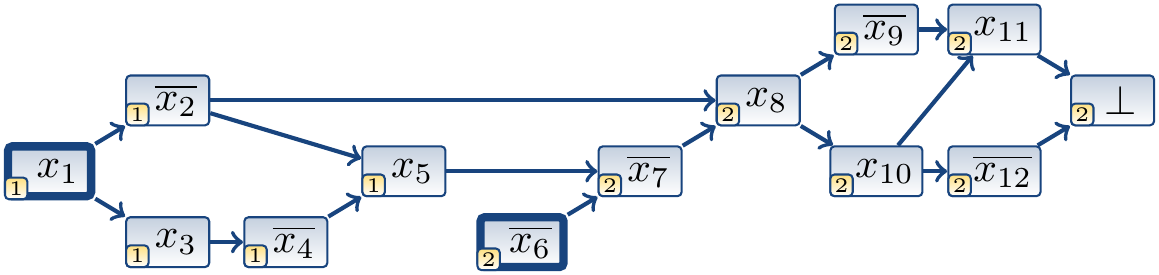
\includegraphics[width=\linewidth]{images/CDCL_1.png}
    \caption{Implication Graph example.\newline (Ref: \url{https://users.aalto.fi/~tjunttil/2022-DP-AUT/notes-sat/cdcl.html})}
    \label{fig:CDCL}
\end{figure}

In our mental model of SAT solving as a tree, let us distinguish between decided variables and unit propagated variables.
In Figure~\ref{fig:CDCL}, the decided variables' cells have a bolded border.
Furthermore, the number in yellow attached to each node tells us when it was decided or unit-propagated.

In that example, we observe that we obtain a contradiction after setting $x_6 = F$ and following some unit propagations.
Furthermore, observe that a cut of the above graph that separates decided variables' nodes from the contradiction node corresponds to a valid clause.

The 1UIP corresponds to the first cut which, after backtracking, yields a unit clause.
This allows us to use our learned clause immediately;
as opposed to choosing some other cut - suppose the one that separates exactly $\bot$, corresponding to the conflict clause $x_{11} \lor x_{12}$ - which is not immediately helpful after backtracking to $x_6$.

To execute this algorithm, we require extra information on variable assignments - when it was assigned, and what clause was used in its unit propagation.
Then, in reverse chronological order, we resolve clauses (see \url{https://en.wikipedia.org/wiki/Resolution_(logic)} for more detail), until the decided variable (in the example $x_6$) is the latest variable assigned.
In this example, the 1UIP cut is the cut exactly to the right of $\overline{x_2}, x_5, \overline{x_6}$, which corresponds to the clause $x_2 \lor \neg x_5 \lor x_6$, which is indeed unit after backtracking once.

There are a few degrees of freedom we can play with here.
Particularly, very large conflict clauses are more likely to be unhelpful than short clauses (indeed, they prune less of the search space).
They also inherently require more effort to track.
Therefore, a variable we optimized over was the maximum limit of allowed conflict clauses.

\subsubsection{Handling Local Conflict Clauses}
It turns out that we can improve over naive backtracking, to something called non-chronological backjumping.
When we derive a conflict clause, after one backtrack, it becomes unit.
However, note that in many cases, we can backtrack many more times without changing its ``unit clause'' status.

For example, consider a derived conflict clause $a \lor b \lor c$, where $a$ was decided on iteration 1, $b$ on 2, and $c$ on 10.
(Note this implies that we are currently on iteration 11, having just erroneously decided $c$.)
We can choose to backtrack back to iteration 10, or consider back\textit{jumping} all the way back to 2, where we unit propagate $c$, then decide a new variable from there.

Indeed, empirically this works a lot better.
Intuitively, it is also not the most surprising.
Now that we have access to the information of $c$ by iteration 3, we minus well use it.
Secondly, this saves us a marginal amount of time of having to unit propagate $c$ repeatedly.
Thirdly, this groups hotly-contested variables close together at the top of the tree, which has a better chance of pruning later parts of our tree.

Recalling our edit stack, adding extra clauses introduces extra complexity.
When we add a conflict clause, we have to also add it to the edit stack in the right locations.
By having each variable maintain a pointer to the correct place in the edit stack, and iterating over relevant variables, we were able to efficiently maintain the validity of our edit stack.

\subsection{Parallel Implementation}

\subsubsection{Work Stealing}

\begin{figure}
    \begin{center}
        \begin{tikzpicture}
            \begin{scope}[every node/.style={circle,thick,draw}]
                \node (R) [draw=red, text=red] at (8, 3) {$S_0$};
                \node (S1T) [draw=red, text=red] at (4, 1) {$S_1$};
                \node (S1F) [dashed, draw=gray, thin, draw=red, text=red] at (12, 1) {$S_1'$} ;
                \node (S2T) [draw=red, thin, text=red] at (2, -1) {$S_2$};
                \node (S2F) at (7, -1) {$S_2'$} ;
                \node (S3T) at (5, -3) {$S_3$};
                \node (S3F) [dashed, draw=gray, thin, text=gray] at (9, -3) {$S_3'$} ;
            \end{scope}
            
            \begin{scope}[
                          every node/.style={fill=white,circle},
                          every edge/.style={draw=black,very thick}]
                \path [->] (R) edge[bend right=20, draw=red, text=red] node {$x_1 = T$} (S1T);
                \path [->] (R) edge[bend left=20, dashed, draw=red, thin, text=red] node {$x_1 = F$} (S1F);
                \path [->] (S1T) edge[bend right=20, draw=red, thin, text=red] node {$x_2 = T$} (S2T);
                \path [->] (S1T) edge[bend left=20, draw=red, text=red] node {$x_2 = F$} (S2F);
                \path [->] (S2F) edge[bend right=20] node {$x_3 = T$} (S3T);
                \path [->] (S2F) edge[bend left=20, dashed, draw=gray, thin, text=gray] node {$x_3 = F$} (S3F);
            \end{scope}
        \end{tikzpicture}
    \end{center}
    \caption{A simple decision tree after having it's work (task $x_1 = F$) stolen}
    \label{fig:dec-tree2}
\end{figure}

In order to parallelize, we want different processes to be working on unique variable assignments. If we statically assign processes their own unique starting set of variables assignments, some may fail rather quickly and be left with no work to do. By allowing for work stealing, we can also simplify the setup by having only PID 0 start with work to do, and the others begin with no work to do, and must steal from PID 0 or some other process. This is also preferable to static assignment at the beginning, since with a static assignment, some variable assignments may be redundant, unit propagated, or already false. With work stealing, we take only tasks that the giving process wasn't sure of, i.e., a variable who's truth status is unknown and was recursed on.

As seen in Figure~\ref{fig:dec-tree2}, task $x_1 = F$ is stolen by some other thread, meaning we can actually prune the top of the tree until it reaches the recursion point of the next task to do or be stolen, which is $S_2'$ here since the next task is $S_3'$.

The oldest compressed version of the formula was originally saved at the state $S_0$ and given to the thief process along with their task. We must then update the oldest compressed formula to be at the top of our new decision tree whose root is now $S_2'$. This is done by applying the all of the edits made between $S_0$ and $S_2'$ to the compressed formula, and discarding these edits afterwards.

\subsubsection{Communication Tree}

\begin{figure}
    \begin{center}
        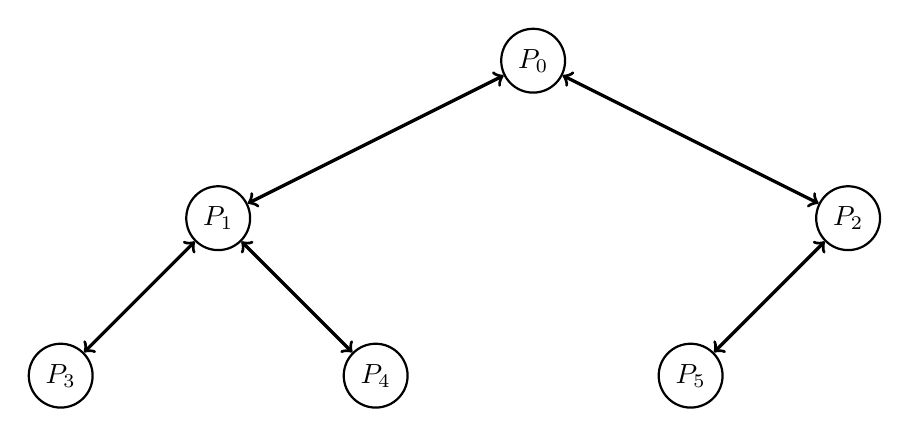
\begin{tikzpicture}
            \begin{scope}[every node/.style={circle,thick,draw}]
                \node (P0) at (8, 4) {$P_0$};
                \node (P1) at (4, 2) {$P_1$};
                \node (P2) at (12, 2) {$P_2$};
                \node (P3) at (2, 0) {$P_3$};
                \node (P4) at (6, 0) {$P_4$};
                \node (P5) at (10, 0) {$P_5$};
            \end{scope}
            \path [<->] (P0) edge[draw=black,very thick] node {} (P1);
            \path [<->] (P0) edge[draw=black,very thick] node {} (P2);
            \path [<->] (P1) edge[draw=black,very thick] node {} (P3);
            \path [<->] (P1) edge[draw=black,very thick] node {} (P4);
            \path [<->] (P2) edge[draw=black,very thick] node {} (P5);
        \end{tikzpicture}
    \end{center}
    \caption{A process tree over 6 threads with branching factor 2}
    \label{fig:proc-tree}
\end{figure}

We now introduce a completely separate tree representing the communication and work stealing restrictions between processes. Each node is a single process who may or may not have work to do, and each process may only communicate with its neighbors (parent or children) with the exception of broadcasting conflict clauses or abort messages. Figure~\ref{fig:proc-tree} shows such a tree with branching factor 2 over 6 threads. In the example, $P_1$ might have work to do but $P_4$ needs work in which case $P_1$ would serve some of its work to $P_4$ via work stealing.

Each process must maintain who's asked them for work (resetting values when they give work), and who they've asked for work (resetting values when they receive work). A process may ask either their children or parent for work, with the order being arbitrary performance-wise. It is important to ensure that processes don't double request the same neighbor for work so as to limit race conditions and free up the interconnect message pipeline.

\subsubsection{Algorithm Termination}

Knowing some processes have work and some don't gives an intuitive graph interpretation of when the algorithm should terminate. First, if some process finds a solution, it will broadcast an abort messages to every other process, ending the algorithm for everyone.

For a process to identify whether the algorithm has failed because everyone is out of work, we need processes to send ``I'm done'' messages to others. Without a tree structure, a process seeing $p - 1$ of these messages would naively believe everyone is done and abort itself. However, we have not guarantee of message fairness with MPI, so it's still possible that there is work in the tree that is sent and not yet received, leading to a false termination. This scenario may arise in any process graph with cycles, where we may also see a more complex race condition in which the algorithm never terminates.

By removing cycles from the process graph (making it an undirected tree), we get a lemma for termination. We call a subtree at some node ``dead'' if the node is out of work and the subtrees rooted at all but one of its neighbors (children or parent) are also dead. If a subtree is dead, we know that there is no work on this tree either at the nodes or along the edges having been sent but not received. This is because a node only knows one of its subtrees is dead via a message from it, which of course would be received after any work sent over that same edge. 

If a subtree is considered dead, it must forward an ``I'm dead'' message to the one remaining neighbor who didn't tell us they were dead. If a process is out of work and it receives these messages from every neighbor, the entire tree must be dead so the process may terminate after forwarding on this message (which makes other neighbors do the same thing).

These special messages indicating a branch is dead should be treated as urgent work requests, taking higher priority for work stealing than normal work requests.

Briefly note that this interconnect structure not having loops (i.e. being a tree) is the key to our termination lemmas to hold.

\subsubsection{Conflict Clause Sharing}

Due to their limited message size and possible usefulness to all other processes, we have the option to broadcast the conflict clauses generated to all other processes.
This introduces more degrees of freedom we can optimize over.
Processing and/or storing irrelevant conflict clauses can turn out to be very costly.
However, because processors can be working under many different contexts, it is possible that a conflict clause they generate would be difficult or impossible for another processor to generate, and thus very useful.
(For example, processor 1 discovers that the second variable it decided, $x_2$ had to be false. This gives every other processor an extra bit of knowledge. We observed several cases where this could invalidate an entire processor's work, as it grabbed work under the context of $x_2 = T$.)

This gave us several variables that we optimized over: how large of a conflict clause to send, and under what circumstances one should keep a remotely-observed conflict clause.
It turns out that conflict clauses should be shared very sparingly, perhaps because each processor is focusing on different parts of search space, and investigating different variables.

If the conflict clause is entirely false, we need to backtrack sufficiently far.
An interesting idea was to do a similar idea to 1UIP, where we would backtrack as few times as possible, then resolve until it is unit.
However, empirically, the extra resolution had very little bearing on the number of iterations required.
Indeed, this could make intuitive sense, as a remote conflict clause will not be as relevant to the context of the current processor.
Therefore, we also decided not to do any backjumping, and stick with the minimal number of backtracks.

\section{Results}
We measured the average time required to solve a suite of 16x16 moderate-level killer sudokus against varying numbers of processors.
Due to the inherent randomness of each processor's speed, the time on a single test case can vary drastically.
A processor can happen to take work which will immediately yield an answer, or the correct answer can be the last leaf of the tree searched.

Another interesting phenomenon when running on $n=1\sim8$ is from the initial distribution of work.
The more processors there are, the more communication time and work stealing happens, which takes more and more time.
However, if processor 1 on $n=4$ vs $n=5$ gets the same work, and no one steals the correct answer from it, then it will require the exact same number of iterations to find the solution.
However, the extra time spent processing others' work requests and conflict clauses slows it down in the latter case.

Therefore, on $n=1,2,4,8,16$ processors, we generated a set of 10 generated killer sudokus, and ran each configuration five times.
For each puzzle, we calculate the average speedup, then averaging over all test cases give the following graph.

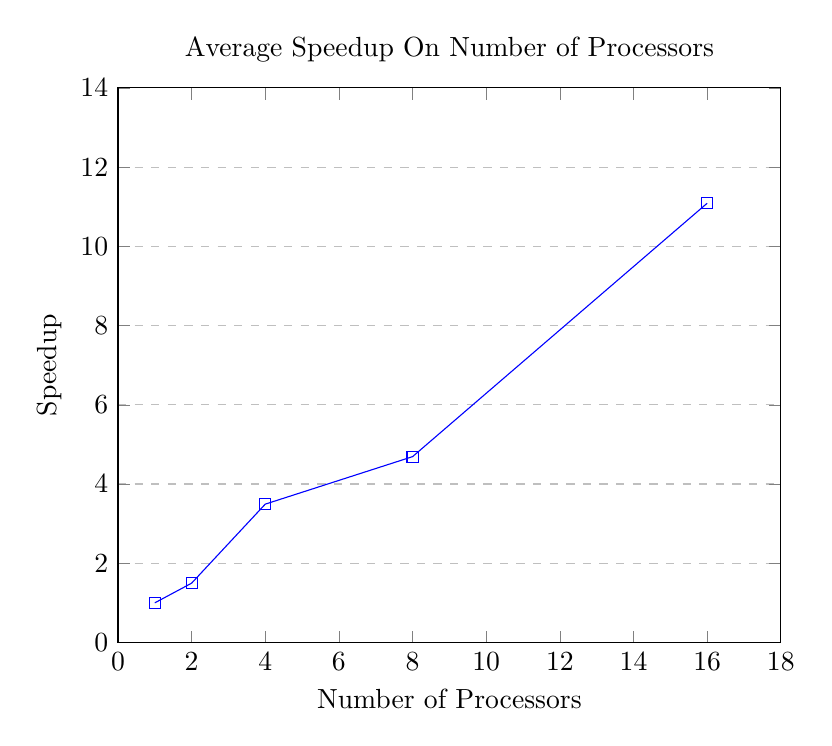
\begin{tikzpicture}
\begin{axis}[
    title={Average Speedup On Number of Processors},
    xlabel={Number of Processors},
    ylabel={Speedup},
    xmin=0, xmax=18,
    ymin=0, ymax=14,
    ymajorgrids=true,
    grid style=dashed,
]
\addplot[
    color=blue,
    mark=square,
    ]
    coordinates {
    (1,1) (2,1.497) (4, 3.492) (8, 4.691) (16,11.088)
    };
    
\end{axis}
\end{tikzpicture}

To also provide an idea to execution time (and the high variance within), we provide the first few per-puzzle data in the table below.
Each number is the five-run average number of seconds it took to solve.

\vspace{12pt}
\begin{tabular}{c|ccccc}
    \hline
    Puzzle Number & $n=1$ & $n=2$ & $n=4$ & $n=8$ & $n=16$ \\
    \hline
    0 & 29.0 & 89.8 & 16.9 & 1.90 & 1.00\\
    1 & 12.69 & 7.81 & 1.35 & 1.70 & 0.89\\
    2 & 23.66 & 14.5 & 6.88 & 3.85 & 2.96\\
    3 & 4.01 & 2.45 & 1.90 & 2.41 & 0.77
\end{tabular}
\label{tab:data}
\vspace{12pt}

\subsection{Testing Configuration}

For our central result, we used the empirically-most optimal settings, to our knowledge.
\begin{itemize}
    \item We kept the maximum conflict clause size to $8n = 128$.
    \item We broadcast conflict clauses only if they were $\leq n=16$ long.
    \item If a remote conflict clause was received, we only kept it if it contained $\leq n/2 = 8$ unassigned variables and wasn't true.
    \item When receiving work, we only kept conflict clauses which contained $\leq 8$ unassigned variables.
    \item Every 100 iterations, we processed messages.
    \item Branching factor to be $n-1$.
\end{itemize}

On our choice of decided variable, the algorithm preferred to pick from a currently small clause which originally contained the most variables.

It turned out to be very difficult to generate good sudokus for this test case.
We need $n=1$ to run in a reasonable amount of time, but not too fast such that additional processors do very little of the work.
Additionally, due to high variance on $n>1$, one can get very lucky or very unlucky, which can range (in one instance) from 0.2 seconds to 480 seconds!
For this reason, I filtered out many puzzles from the generator that took $n=1$ under 2 seconds or over 2 minutes.
Under such restrictions, we generated 10 test cases which are 16x16 killer sudokus with max cage size of 4.
For reference, these have roughly $12500$ variables and $56000$ clauses.

\subsection{Discussion}

Due to the algorithm overall slow speed before optimizations, we initially tested only on blank Sudoku grids since they were the only ones where the algorithm could terminate in reasonable time. Blank grids require little backtracking, so it's possible to terminate very fast by making optimal assignment decisions. 

As we neared the completion of the core recursive algorithm following the checkpoint, there was concern as to whether the search problem made the most sense in a parallel context. Consider an analogy where each process is an athlete racing each other to the finish line to find the solution. With the work-stealing model, we see $P_0$ actually gets to start first, and that other processes only actually take sidelined work. This is even worse with the blank grids, as $P_0$ becomes the fastest runner in the world for any process count, ruining any chance of parallelism as the other processes take sub-optimal decisions as their work. Even with conflict resolution and sharing, we see slow processes give $P_0$ redundant conflict clauses. This is like one of the slow racers shouting to Usain Bolt to watch out for a hole in the ground that he already passed several minutes ago. 

Without artificially making processes make sub-optimal decisions (which would make it infeasibly-long), we needed harder test cases. Indeed, solving blank Sudoku's (i.e., generating a solution) isn't an interesting or long problem to solve. With the killer variant and some filled-in values, there is much more backtracking required. It's no-longer guaranteed that $P_0$ or work-giving process makes better decisions than it's stealing children. 

In our final algorithm, the process that finds the solution first is basically up to the chance of race conditions for work stealing. There's a good amount of variance in this, so in our performance and speedup testing, we average over several iterations.

Over the period where no speedup was seen due to blank input grids, it seemed as though the better way to parallelize would have been to split the work done rather than the search space. This would be a single (or just a few) instance(s) of the search algorithm making use of several threads to do expensive loop or bulk updates required. These kinds of updates are all over DPLL, such as the unit prop, which may involve updating many clauses and variables independently at the same time. Surely on an RTX 2080 GPU, the actual work done by the algorithm could be almost perfectly split. 

Having seen some of our processes making useless contributions to the problem at the time, the GPU approach seemed like the one we should have started with. However, we know at this point there are instances of possible super-linear speedup when it comes to paralleling over the search space. 

Consider a contrived input example where SAT variable $x_1$ must always be false in every valid solution, but this fact is not discovered until deep within the search tree. Now suppose we begin by trying $x_1 = T$ on a single process. Assuming no conflict learning, the single process must search the entire search space before backtracking to $x_1 = F$. Under even small test cases, this search space exceeds the number of particles in the known universe, whereas some $P_1$ could just steal $x_1 = F$ and terminate instantly. Of course with conflict learning (or some kind of memorization), this doesn't happen in practice. What does happen is $P_1$ would have a massive head start over $P_0$, who has to run into the error, and derive several conflict clauses just to reach the conclusion another thread started with.

We get even better parallelism considering processes that make early mistakes share conflict clauses to processes who may need them but have not yet lived this mistake. These received conflict clauses may just appear always false for a process from the beginning of their work, in which case we've pruned the entire bottom of a search tree, and the receiving process can just dump their work and steal more.

We chose to include the following table to discuss some interesting empirical results of branching factor.
These were averaged over three runs on the 8th test case with 2 processors.
In the following table, we look at the per-puzzle speedup of $n=8$ with branching factor 2 vs 7.

\vspace{12pt}
\begin{tabular}{c|cc}
    \hline
    Puzzle Number & $b=2$ speedup & $b=7$ speedup\\
    \hline
    0 &3.40 & 15.27\\
    1 &4.27 & 3.90\\
    2 &5.15 & 7.47\\
    3 &0.75 & 0.80\\
    4 &0.37 & 3.12\\
    5 &0.41 & 0.12\\
    6 &1.86 & 1.79\\
    7 &6.32 & 6.15\\
    8 &9.86 & 2.74\\
    9 &2.34 & 1.66\\
    \hline
    average & 3.47 & 4.69
\end{tabular}
\label{tab:bf}
\vspace{12pt}

Interestingly enough, in this second testrun, the average $n=4$ speedup was 3.81, which is higher than $n=8$'s.

A priori, we thought having the branching factor of 2 to be ideal.
However, when we had the thought that perhaps work was taking too long to traverse the whole tree, and using a branching factor of $n-1$, we found a surprising non-trivial speedup.
In exchange for overburdening one processor with handling most of the communication, it seems that the work was distributed more efficiently.
Indeed, if we consider the worst case scenario where one leaf processor (w.r.t the process tree) has the last remaining work, it takes a lot of messages to get some work to an idle processor on the far end of the tree!
That being said, on very high processor counts, it should be consider having a higher depth process tree [than 2], to limit the traffic bottleneck around the one root node.

\begin{figure}
    \centering
    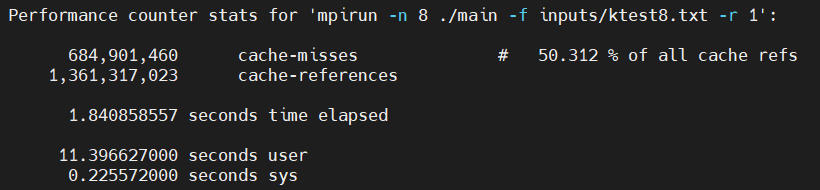
\includegraphics[width=1\linewidth]{images/perf1.png}
    \caption{Perf stat on $n=8$ for cache-references and cache-misses.}
    \label{fig:perf1}
\end{figure}

\begin{figure}
    \centering
    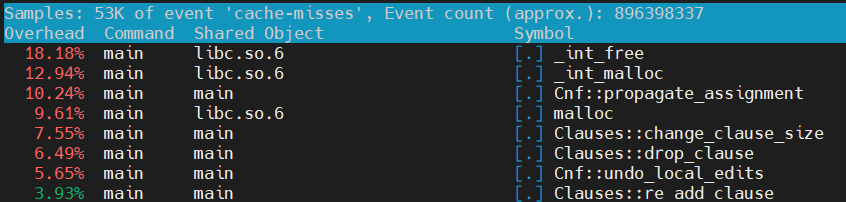
\includegraphics[width=\linewidth]{images/perf2.png}
    \caption{Perf report on $n=8$ for cache-misses}
    \label{fig:perf2}
\end{figure}

\begin{figure}
    \centering
    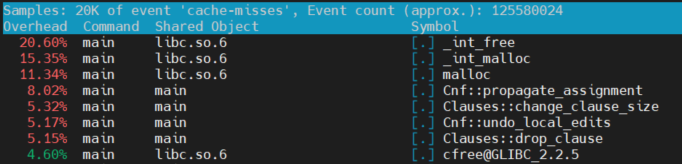
\includegraphics[width=1\linewidth]{images/perf_n1.png}
    \caption{Perf report on $n=1$ for cache-misses}
    \label{fig:perf3}
\end{figure}

One of the biggest problems impacting parallelism is cache misses.
In both Figures \ref{fig:perf1} and \ref{fig:perf2}, we observe an extraordinarily high miss rate.
This is as compared to $n=1$, which hovered around a much superior 4.5\%.
Indeed, interestingly the perf report was structured very similar to $n=8$'s, however we note that in the parallel case, the function \verb|reconstruct_state| is called whenever work is stolen.
This decompresses the message (containing variable assignments and dropped clauses) into the State structure.
Indeed, the more work is stolen yields more calls to this function, which in turn calls the functions in Figure \ref{fig:perf2} many times.

Therefore, any slight improvement (in terms of cache locality) to \verb|reconstruct_state| or it's called functions would have an outsized impact on cache misses.
One such improvement is our implementation of the edit stack.
Currently, one edit occupies the entire value of an edit stack element.
However, if we instead had the edit stack hold multiple edits (how many would be another variable to optimize), then we would reduce the number of stack pointers we have to follow.

\section{References}

\begin{itemize}
    \item 
\url{https://www.cs.cmu.edu/~wklieber/papers/2007_efficient-cnf-encoding-for-selecting-1.pdf}
    \item
\url{https://users.aalto.fi/~tjunttil/2022-DP-AUT/notes-sat/cdcl.html}
    \item
\url{https://uva-kr16.github.io/KilerSudoku/paper.pdf}
\end{itemize}

\section{Work Distribution}

\subsection{Overall Work Split}

Factoring in all of the below paired with time spent on the project, the distribution of credit should be a perfect 50\%-50\% split.

\subsection{Liam Work Completion}
\begin{itemize}
    \item Message passing infrastructure (interconnect)
    \item Core recursive DPLL algorithm
    \item Work stealing design and implementation
    \item Parallel communication and termination implementation
    \item Underlying data structures for formula
    \item Formula compression work
    \item Version control
\end{itemize}

\subsection{Alexander Work Completion}

\begin{itemize} 
    \item Sat reductions
    \item Conflict Resolution implementation
    \item Conflict Clause Sharing
    \item Backtracking logic
    \item Edit history logic
    \item Debugging of race conditions
    \item Killer Variant of Sudoku
    \item Writing test cases
    \item Performance Testing Code
    \item All work on PSC machines
\end{itemize}

\end{document}
